\documentclass[
	12pt,				% tamanho da fonte
	oneside,			% para impressão no anverso. Oposto a twoside
	a4paper,			% tamanho do papel. 
	chapter=TITLE,		% títulos de capítulos convertidos em letras maiúsculas
	section=TITLE,		% títulos de seções convertidos em letras maiúsculas
	english,			% idioma adicional para hifenização
	brazil  			% o último idioma é o principal do documento
	]{abntex2}

\usepackage{setup/ufscthesisA4-alf}
\usepackage{csquotes}
\usepackage[backend = biber, style = abnt]{biblatex}
\usepackage{graphicx}
\usepackage{color}
\usepackage{listings}
\usepackage{multirow}
\usepackage{tabularx}
\usepackage[table]{xcolor}
\usepackage{colortbl}
\usepackage{framed}
\usepackage{amssymb}
\usepackage{afterpage}
\usepackage{hhline}
\usepackage{enumitem}
\usepackage{latexsym}
\usepackage{lipsum}
\usepackage{setspace}
\usepackage{tabularray}

\definecolor{shadecolor}{rgb}{0.8,0.8,0.8}

\setlength\bibitemsep{\baselineskip}
\DeclareFieldFormat{url}{Disponível~em:\addspace\url{#1}}
\NewBibliographyString{sineloco}
\NewBibliographyString{sinenomine}
\DefineBibliographyStrings{brazil}{%
	sineloco     = {\mkbibemph{S\adddot l\adddot}},
	sinenomine   = {\mkbibemph{s\adddot n\adddot}},
	andothers    = {\mkbibemph{et\addabbrvspace al\adddot}},
	in			 = {\mkbibemph{In:}}
}

\addbibresource{aftertext/references.bib}

\DeclareSourcemap {
	\maps[datatype=bibtex] {
		\map {
			\step[fieldset=abstract, null]
			\step[fieldset=pagetotal, null]
		}
		\map {
			\pertype{inproceedings}
			\step[fieldset=venue, null]
			\step[fieldset=eventdate, null]
			\step[fieldset=eventtitle, null]
			\step[fieldset=isbn, null]
			\step[fieldset=volume, null]
		}
	}
}

% Definições gerais
\autor{Eric Fernandes Evaristo}
\titulo{Uso de uma MLLM para classificar lesões de pele}
\orientador[Orientador]{Aldo von Wangenheim, Prof. Dr. rer.nat.}  % TODO: Verificar os títulos
\ano{2024}
\local{Florianópolis}
\instituicaosigla{UFSC}
\instituicao{Universidade Federal de Santa Catarina}
\tipotrabalho{Proposta de Trabalho de Conclusão de Curso}
\formacao{Bacharel em Ciências da Computação}
\nivel{Bacharel}
\programa{Curso de Graduação em Ciências da Computação}
\centro{Centro Tecnológico}

\preambulo {
	\imprimirtipotrabalho~do~\imprimirprograma~do~\imprimircentro~da~\imprimirinstituicao~para~a~obtenção~do~título~de~\imprimirformacao.
}

% Configurações de aparência do PDF final
\definecolor{blue}{RGB}{41,5,195}
\makeatletter
\hypersetup{
		pdftitle={\@title},
		pdfauthor={\@author},
    	pdfsubject={\imprimirpreambulo},
	    pdfcreator={LaTeX with abnTeX2},
		pdfkeywords={ufsc, latex, abntex2},
		colorlinks=true,
    	linkcolor=black,
    	citecolor=black,
    	filecolor=black,
		urlcolor=black,
		bookmarksdepth=4
}
\makeatother

% Declaração das siglas
\siglalista{MLLM}{\textit{Multimodal Large Language Model}}
\siglalista{MLLMs}{\textit{Multimodal Large Language Models}}
\siglalista{LLM}{\textit{Large Language Model}}
\siglalista{LLMs}{\textit{Large Language Models}}
\siglalista{LLaVA}{\textit{Large Language and Vision Assistant}}
\siglalista{LLaMA 3.2}{\textit{Large Language Model Meta AI}}
\siglalista{CLIP ViT-L/14}{\textit{Contrastive Language-Image Pre-training ViT-L/14}}
\siglalista{PEFT}{\textit{Parameter-Efficient Fine-Tuning}}
\siglalista{LoRa}{\textit{Low-Rank Adaptation}}
\siglalista{QLoRa}{\textit{Quantized Low Rank Adaptation}}
\siglalista{TCC}{Trabalho de Conclusão de Curso}
\siglalista{CPNM}{cânceres de pele não melanoma}
\siglalista{CBC}{carcinoma basocelular}
\siglalista{CEC}{carcinoma epidermoide}

% Compila a lista de abreviaturas e siglas e a lista de símbolos
\makenoidxglossaries

% Compila o indice
\makeindex

% Início do documento
\begin{document}

% Seleciona o idioma do documento (conforme pacotes do babel)
\selectlanguage{brazil}

% Retira espaço extra obsoleto entre as frases.
\frenchspacing

% Espaçamento 1.5 entre linhas
\OnehalfSpacing

% Elementos pré-textuais
% Capa
\imprimircapa

% Folha de rosto
% (o * indica que haverá a ficha bibliográfica)
\imprimirfolhaderosto

% Folha de aprovação
\begin{folhadeaprovacao}
	\small
	\begin{snugshade}
		\begin{center}
			{\textbf{FOLHA DE APROVAÇÃO DE PROPOSTA DE TCC}}
		\end{center}
	\end{snugshade}
	\vspace{-18pt}

	\footnotesize
	\begin{quadro}[htb]
		\centering
		\label{qua:folha_aprov}
		\begin{tabular}{|l|p{10.5cm}|}
			\hline
			\textbf{Acadêmico}            & \imprimirautor      \\ \hline
			\textbf{Título do trabalho}   & \imprimirtitulo     \\ \hline
			\textbf{Curso}                & \imprimirprograma   \\ \hline
			\textbf{Área de Concentração} & Visão computacional \\ \hline
		\end{tabular}
	\end{quadro}

	\vspace{-14pt}

	\noindent \textbf{Instruções para preenchimento pelo ORIENTADOR DO TRABALHO}:
	\begin{itemize}[leftmargin=*,noitemsep,topsep=0pt]
		\item[-] Para cada critério avaliado, assinale um X na coluna SIM apenas se considerado aprovado. Caso contrário, indique as alterações necessárias na coluna Observação.
	\end{itemize}

	\vspace{-4pt}

	\definecolor{Silver}{rgb}{0.752,0.752,0.752}
	\begin{table}[htb]
		\footnotesize
		\centering
		\begin{tblr}{
			width = \linewidth,
			colspec = {Q[452]Q[56]Q[85]Q[56]Q[150]Q[137]},
			row{1} = {Silver,c},
			row{2} = {Silver,c},
			cell{1}{1} = {r=2}{},
			cell{1}{2} = {c=4}{0.347\linewidth},
			cell{1}{6} = {r=2}{},
			cell{3}{2} = {Silver},
			cell{3}{3} = {Silver},
			cell{3}{4} = {Silver},
			cell{3}{5} = {Silver},
			cell{4}{2} = {Silver},
			cell{4}{3} = {Silver},
			cell{4}{4} = {Silver},
			cell{4}{5} = {Silver},
			cell{5}{2} = {Silver},
			cell{5}{3} = {Silver},
			cell{5}{4} = {Silver},
			cell{5}{5} = {Silver},
			cell{6}{2} = {Silver},
			cell{6}{3} = {Silver},
			cell{6}{4} = {Silver},
			cell{6}{5} = {Silver},
			cell{7}{2} = {Silver},
			cell{7}{3} = {Silver},
			cell{7}{4} = {Silver},
			cell{7}{5} = {Silver},
			cell{8}{2} = {Silver},
			cell{8}{3} = {Silver},
			cell{8}{4} = {Silver},
			cell{8}{5} = {Silver},
			cell{9}{2} = {Silver},
			cell{9}{3} = {Silver},
			cell{9}{4} = {Silver},
			cell{9}{5} = {Silver},
			cell{10}{2} = {Silver},
			cell{10}{3} = {Silver},
			cell{10}{4} = {Silver},
			cell{10}{5} = {Silver},
			cell{11}{2} = {Silver},
			cell{11}{3} = {Silver},
			cell{11}{4} = {Silver},
			cell{11}{5} = {Silver},
			cell{12}{2} = {Silver},
			cell{12}{3} = {Silver},
			cell{12}{4} = {Silver},
			cell{12}{5} = {Silver},
			cell{13}{2} = {Silver},
			cell{13}{3} = {Silver},
			cell{13}{4} = {Silver},
			cell{13}{5} = {Silver},
			cell{14}{2} = {Silver},
			cell{14}{3} = {Silver},
			cell{14}{4} = {Silver},
			cell{14}{5} = {Silver},
			cell{15}{2} = {Silver},
			cell{15}{3} = {Silver},
			cell{15}{4} = {Silver},
			cell{15}{5} = {Silver},
			vlines,
			hline{1,3-16} = {-}{},
					hline{2} = {2-5}{},
				}
			\textbf{Critérios }                                                                                                                                                                                                                                                                                & \textbf{Aprovado } &                  &              &                        & \textbf{Observação } \\
			                                                                                                                                                                                                                                                                                                   & \textbf{Sim}       & \textbf{Parcial} & \textbf{Não} & \textbf{Não se aplica} &                      \\
			{1. O trabalho é adequado para um TCC no CCO/SIN (relevância / abrangência)?}                                                                                                                                                                                                                      &                    &                  &              &                        &                      \\
			2. O titulo do trabalho é adequado?                                                                                                                                                                                                                                                                &                    &                  &              &                        &                      \\
			{3. O tema de pesquisa está claramente descrito?}                                                                                                                                                                                                                                                  &                    &                  &              &                        &                      \\
			{4. O problema/hipóteses de pesquisa do trabalho está claramente identificado?}                                                                                                                                                                                                                    &                    &                  &              &                        &                      \\
			5. A relevância da pesquisa é justificada?                                                                                                                                                                                                                                                         &                    &                  &              &                        &                      \\
			{6. Os objetivos descrevem completa e claramente o que se pretende alcançar neste trabalho?}                                                                                                                                                                                                       &                    &                  &              &                        &                      \\
			{7. É definido o método a ser adotado no trabalho? O método condiz com os objetivos e é adequado para um TCC?}                                                                                                                                                                                     &                    &                  &              &                        &                      \\
			{8. Foi definido um cronograma coerente com o método definido (indicando todas as atividades) e com as datas das entregas (p.ex. Projeto I, II, Defesa)?}                                                                                                                                          &                    &                  &              &                        &                      \\
			{9. Foram identificados custos relativos à execução deste trabalho (se houver)? Haverá financiamento para estes custos?}                                                                                                                                                                           &                    &                  &              &                        &                      \\
			{10. Foram identificados todos os envolvidos neste trabalho?}                                                                                                                                                                                                                                      &                    &                  &              &                        &                      \\
			{11. As formas de comunicação foram definidas (ex: horários para orientação)?}                                                                                                                                                                                                                     &                    &                  &              &                        &                      \\
			{12. Riscos potenciais que podem causar desvios do plano foram identificados?}                                                                                                                                                                                                                     &                    &                  &              &                        &                      \\
			{13. Caso o TCC envolva a produção de um software ou outro tipo de produto e seja desenvolvido também como uma atividade realizada numa empresa ou laboratório, consta da proposta uma declaração (Anexo 3) de ciência e concordância com a entrega do código fonte e/ou documentação produzidos?} &                    &                  &              &                        &
		\end{tblr}
	\end{table}

	\vspace{-4pt}

	\tiny
	\noindent \begin{tabularx}{\textwidth}{| l | X | l | l |}
		\hline
		{\textbf{Avaliação}}     & \multicolumn{1}{l}{\textbf{$\Box$ Aprovado}} & \multicolumn{2}{c|}{\textbf{$\Box$ Não Aprovado}}   \\ \hline
		{\textbf{Orientador}}    & {Prof. Dr. rer.nat. Aldo von Wangenheim}     & {00/00/2024}                                      & \\ \hline
		{\textbf{Co-orientador}} & {-}                                          & {00/00/2024}                                      & \\ \hline
	\end{tabularx}
\end{folhadeaprovacao}

% Resumo em português
\setlength{\absparsep}{18pt}
\begin{resumo}
	\SingleSpacing

	Lesões de pele podem ser um indicativo de diversas doenças, incluindo doenças graves como o câncer de pele. A detecção precoce dessas lesões é fundamental para o
	tratamento e cura da doença. Porém, o diagnóstico e classificação de uma lesão de pele é normalmente feita por profissionais especializados em hospitais ou clínicas.
	Isto pode levar a um atraso no diagnóstico pela falta de acesso ou procura pelo atendimento médico.

	Considerando este cenário, tecnologias como \ac{MLLMs} podem ser úteis. Estes modelos podem identificar lesões de pele com base em imagens e prover um pré-diagnóstico
	que pode alertar o portador da lesão sobre a necessidade de procurar atendimento médico. O modelo \ac{LLaVa} é um bom candidato para esta aplicação, pois consegue
	descrever imagens e pode ser adaptado para propósitos específicos.

	Neste trabalho, propõe-se a adaptação do \ac{LLaVa} com técnicas de \textit{fine tuning} para classificar lesões de pele com uma precisão aceitável.

	\textbf{Palavras-chave:} Lesões de pele. MLLM. LLaVa. Fine tuning. PEFT.
\end{resumo}

% Resumo em inglês (TODO)
%\begin{resumo}[Abstract]
%	\SingleSpacing
%	\begin{otherlanguage*}{english}
%		Resumo traduzido para outros idiomas, neste caso, inglês. Segue o formato do resumo feito na língua vernácula. As palavras-chave traduzidas, versão em língua estrangeira, são colocadas abaixo do texto precedidas pela expressão “Keywords”, separadas por ponto.

%		\textbf{Keywords}: Keyword 1. Keyword 2. Keyword 3.
%	\end{otherlanguage*}
%\end{resumo}

{
\hypersetup{hidelinks}

% Lista de siglas
\imprimirlistadesiglas

% Sumário
\pdfbookmark[0]{\contentsname}{toc}
\tableofcontents*
\cleardoublepage
}


% Elementos textuais
\textual

% 1 - Introdução
\chapter{Introdução}

Lesões de pele são indicativos de diversas doenças, como infecções de baixo risco ou até mesmo câncer. Cerca de 30\% dos tumores malignos registrados no Brasil são
causados pelo câncer de pele \cite{skin_cancer_in_brazil}. Os tipos mais comuns desta doença são o carcinoma basocelular e o carcinoma epidermoide, que mesmo tendo uma
baixa letalidade, podem causar sequelas expressivas por conta do tratamento. O melanoma é o menos frequente, mas possui uma letalidade muito maior, causando 75\% das mortes
por câncer de pele \cite{skin_cancer_screening}.

A detecção precoce do câncer de pele é essencial para a garantia da efetividade do tratamento, pois a taxa de sobrevida dos pacientes tende a cair ao longo do avanço
da doença \cite{skin_cancer_survival}. Observa-se que indivíduos com um grau menor de escolaridade têm um prognóstico pior, pois apresentam tumores em estágios mais
avançados \cite{skin_cancer_socioeconomic}. Esta correlação pode indicar que a falta de conhecimento sobre a doença ou problemas socioeconômicos podem resultar no atraso
do diagnóstico e consequentemente na redução da taxa de sucesso do tratamento.

Considerando este cenário, o desenvolvimento de um sistema automatizado de fácil utilização de classificação de lesões de pele pode ser útil na identificação precoce de
melanomas e outros tipos de doenças. \ac{MLLMs} conseguem obter uma precisão significativa na classificação de imagens de diagnósticos médicos, o que torna viável
o uso destes modelos para o desenvolvimento deste trabalho \cite{mllm_success_rate}.

O \ac{LLaVA} foi escolhido como o modelo base devido à limitação de recursos para o treinamento de um novo modelo e por ter o código disponível publicamente. Este
modelo combina o codificador visual \ac{CLIP ViT-L/14} e o \ac{LLM} \textit{Vicuna} \cite{llava}.

Com este modelo, é possível realizar um \textit{fine-tuning}, adaptando-o para a classificação de lesões de pele e principalmente para a detecção de câncer de pele. Com
o objetivo utilizar os recursos computacionais disponíveis eficientemente, o \textit{fine-tuning} será feito com técnicas baseadas em \ac{PEFT}. Este método permite a
redução do número de parâmetros usados no processo, resultando em uma utilização menor de recursos \cite{peft}. Especificamente, planeja-se utilizar métodos como
\ac{LoRa} e \ac{QLoRa} para a adaptação do modelo.

Com as adaptações feitas no \ac{LLaVA}, espera-se obter um sistema confiável de classificação de lesões de pele.

\section{Objetivos}

O objetivo deste trabalho é desenvolver um sistema de classificação de lesões de pele com um foco na detecção de câncer de pele utilizando um \ac{LLM} multimodal.
Serão utilizados métodos de \textit{fine-tuning} para adaptar o modelo base. Além disso, planeja-se analisar a eficiência entre diferentes técnicas de adaptação.

\subsection*{Objetivos Específicos}

\begin{itemize}
    \item Avaliar a eficiência de diferentes métodos de \textit{fine-tuning} e a precisão dos modelos resultantes;
    \item Obter um modelo adaptado que possua uma precisão satisfatória na classificação de lesões de pele e detecção de câncer de pele;
    \item Comparar o modelo adaptado com outros \ac{MLLMs}.
\end{itemize}


% 2 - Capítulo 2
\chapter{Fundamentação Teórica}

% TODO: Atualizar isso aqui
Neste capítulo serão discutidos os aspectos relacionados à classificação de imagens de lesões de pele e detecção de melanomas. Além disso, serão explicados os conceitos
de visão computacional com redes neurais, \acp{LLM} e como estas tecnologias se integram em um \ac{MLLM}. Por fim, será discutido sobre diferentes métodos de
\textit{fine-tuning}.

\section{Lesões de Pele}

A pele é o maior órgão do corpo humano e é responsável por proteger o corpo de agentes microbiológicos, físicos e químicos. Além disso, ela também ajuda na regulação da
temperatura do corpo e, através de receptores cutâneos, proporciona informações sensoriais como o tato \cite{skin}.

Devido à exposição da pele ao ambiente, é mais comum que esse órgão sofra com doenças. As áreas afetadas são consideradas lesões de pele e podem ser usadas para
diagnósticos \cite{segmentation_skin_lesions}.

\subsection{Câncer de Pele}

O câncer é uma doença caracterizada pela multiplicação de células anormais que podem se espalhar para além do seu tecido de origem, causando tumores e levando
eventualmente à morte \cite{cancer}. O câncer de pele é o tipo mais comum da doença globalmente e é mais frequentemente causado pela exposição prolongada à radiação
ultravioleta \cite{skin_cancer}. Em geral, essa doença afeta mais a pele clara e pode afetar a mesma pessoa mais de uma vez. Uma vez desenvolvido, há um aumento de 35\%
no risco de desenvolvimento de um novo câncer de pele do mesmo tipo em um período de três anos \cite{skin_cancer_zink}.

Existem várias categorias de câncer de pele, elas podem ser agrupadas como \ac{CPNM} e melanoma. \ac{CPNM} podem ser subdivididos em \ac{CBC}, \ac{CEC}, carcinoma de
Merkel e entre outros. Essa categoria é a mais incidente, correspondendo a mais de 90\% dos cânceres diagnosticados e também é a menos fatal. O subtipo \ac{CBC} é o
mais frequente e corresponde a mais de 75\% dos casos de \ac{CPNM} no Brasil \cite{skin_cancer_zink}. O melanoma é o tipo mais fatal e menos incidente da doença. Cerca
de 75\% das mortes por câncer de pele são causadas por melanomas \cite{skin_cancer_screening}.

A doença tem um prognóstico muito melhor quando a detecção e tratamento são feitos cedo o suficiente. Segundo \textcite{skin_cancer_survival}, a taxa de sobrevivência ao
melanoma no Brasil é menor que a taxa global, sendo que há uma prevalência maior de casos avançados.

\subsection{Imagens de Lesões de Pele}

As imagens para exames dermatológicos podem ser agrupadas em diferentes categorias. Alguns exemplos baseados em procedimentos recomendados por
\textcite{fotos_dermatologia} são:

% TODO: Adicionar imagens

\begin{itemize}
      \item \textbf{Dermatoscopia}: Essas imagens são obtidas com um equipamento especializado, o dermatoscópio. Esse método permite que um diagnóstico mais preciso seja
            feito, sendo melhor que o olho nu na detecção de melanomas \cite{dermatoscopy}.
      \item \textbf{Foto de aproximação com régua}: Esse tipo de imagem é obtida com uma fotografia feita a 30 centímetros da lesão, sem utilizar \textit{zoom}.
            Nessas imagens, etiquetas são colocadas próximas à lesão para auxiliar na determinação do seu tamanho.
      \item \textbf{Foto panorâmica}: Nesse método são registradas imagens de regiões do corpo, como da cabeça, tronco, braços e pernas.
\end{itemize}

\subsection{Detecção e Diagnóstico de Câncer de Pele}

O câncer de pele pode ser identificado e classificado através dos sintomas causados. Características como o tamanho da lesão, variação da cor, irregularidade do formato,
progresso ao longo do tempo e local do corpo em que a lesão se encontra são fundamentais para o diagnóstico da doença \cite{recognizing_skin_cancer}.

A análise destes sintomas é normalmente um processo visual realizado por um dermatologista, sendo que técnicas como a dermatoscopia e teledermatologia podem ser usadas.
Outros métodos não invasivos incluem, por exemplo, a análise intracutânea espectrofotométrica, ultrasonografia de alta frequência e microscopia confocal de refletância.
É possível também diagnosticar a doença através de métodos invasivos como a biópsia. Além destes métodos, há também a utilização de \ac{IA}. Soluções com \ac{IA}
utilizam imagens para a classificação da doença e podem ter uma precisão equiparável ou até maior a de dermatologistas \cite{recognizing_skin_cancer, skin_cancer_ai}.

\section{Multimodal Large Language Models}

\acp{MLLM} são \acp{IA} baseadas em \acp{LLM} que possuem a capacidade de interpretação de diferentes modalidades de informação, diferentemente de \acp{LLM}, que
operam sobre informações textuais. Esses modelos também podem ser capazes de produzir conteúdo multimodal. Essas modalidades podem ser imagens, vídeos, áudios e
entre outros \cite{mllm_survey_2023, mllm_survey_2024}.

Segundo \textcite{mllm_survey_2024}, a estrutura de um \ac{MLLM} pode ser dividida em cinco componentes, sendo eles o codificador de modalidade, projetor de entrada,
\ac{LLM}, projetor de saída e o gerador de modalidade. No caso de \acp{MLLM} que possuem apenas saída de texto, somente os três primeiros componentes estão presentes,
essa estrutura é demonstrada na \autoref{fig:mllm_structure_encoder_only}.

\begin{figure}[ht]
      \centering
      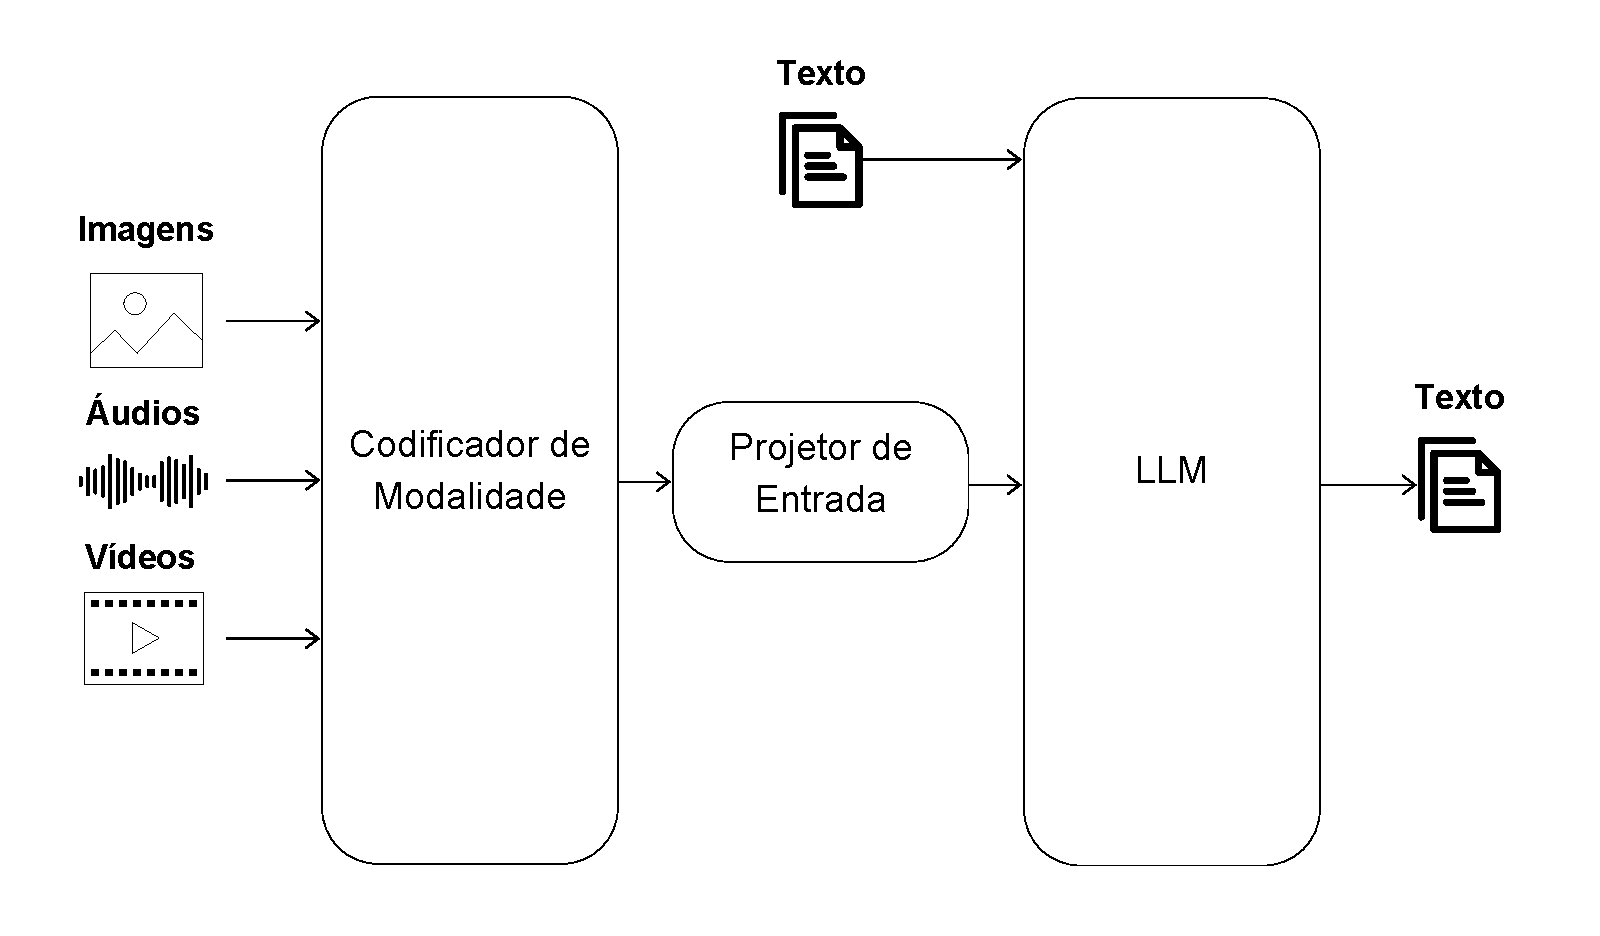
\includegraphics[width=0.7\columnwidth,keepaspectratio]{images/mllm_structure_encoder_only.pdf}
      \caption{\small Estrutura de um \ac{MLLM} que realiza apenas a interpretação multimodal.}
      \label{fig:mllm_structure_encoder_only}
\end{figure}

Neste trabalho, o foco será dado a modelos que interpretam imagens e retornam saídas textuais. Sendo assim, a parte de geração multimodal não será coberta.

\subsection{Large Language Models}

\acp{LLM} ou Grandes Modelos de Linguagem são modelos estatísticos pré-treinados baseados em transformadores capazes de processar e gerar textos em linguagem natural.

\subsubsection{Transformadores}

\subsubsubsection{Incorporação Vetorial}

Um \textit{embedding vector} ou uma incorporação vetorial é um vetor de valores reais em um espaço semântico n-dimensional que representa um dado, como, por exemplo, uma
palavra ou uma imagem. Esse tipo de representação permite que diferentes tipos de dados sejam representados em um espaço vetorial unificado. Na
\autoref{fig:word_embeddings} há um exemplo simplificado da estrutura destes vetores \cite{word_embedding, mllm_survey_2023}.

\begin{figure}[ht]
      \centering
      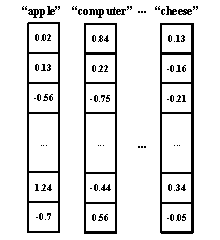
\includegraphics[width=0.4\columnwidth,keepaspectratio]{images/word_embeddings.pdf}
      \caption{\small Representação de palavras como vetores de valores reais. Fonte: \textcite{word_embedding}.}
      \label{fig:word_embeddings}
\end{figure}

Nesse espaço vetorial, direções podem ter um significado semântico. Um exemplo dado por \textcite{glove} demonstra isso com uma frase, traduzida do inglês: "Um rei é para
uma rainha o que um homem é para uma mulher", que pode ser representada como \textit{$V_{rei} - V_{rainha} \approx V_{homem} - V_{mulher}$}, evidenciando que a direção do
vetor \textit{$V_{rei} - V_{rainha}$} codifica informações sobre gênero. Além disso, a proximidade entre incorporações indica a similaridade semântica entre elas. Mais
exemplos dessa relação entre palavras podem ser vistos na \autoref{fig:word_embeddings_directions}.

\begin{figure}[ht]
      \centering
      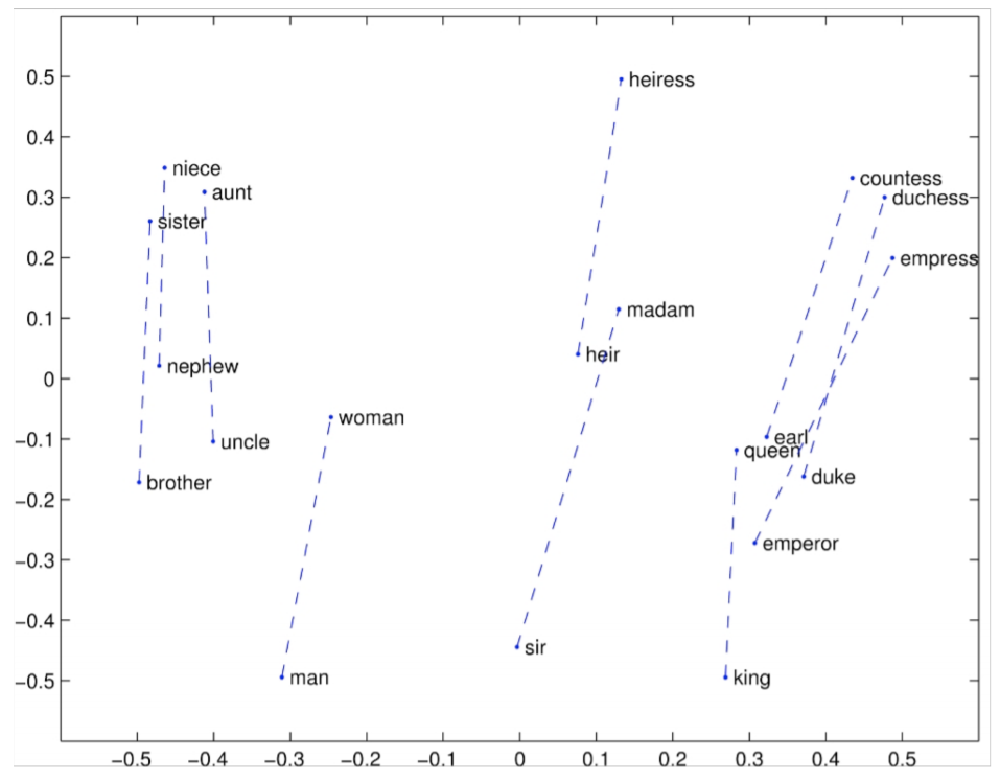
\includegraphics[width=0.7\columnwidth,keepaspectratio]{images/word_embeddings_directions.png}
      \caption{\small Visualização de incorporações com a direção que codifica informações de gênero evidenciada. Fonte: \textcite{word_embedding}.}
      \label{fig:word_embeddings_directions}
\end{figure}
\clearpage  % TODO: Apagar isso aqui se possível

\subsection{Codificador de Modalidade}

Codificadores de modalidade são os componentes responsáveis pela extração das características mais relevantes dos dados multimodais de entrada em incorporações vetoriais.
\cite{mllm_survey_2024}.

\subsubsection{Codificador Visual}

Existem diversos tipos de codificadores visuais. Os mais comuns usam \acp{ViT} ou Transformadores Visuais na suas arquiteturas, mas também há também codificadores
baseados em convolução \cite{mllm_survey_2023}. Neste trabalho o foco será direcionado a arquiteturas baseadas em \ac{ViT}.

\subsubsubsection{Transformadores Visuais}

\subsection{Projetor de Entrada}

\section{Fine-tuning}

\section{LLaMA}


% 3 - Capítulo 3
% % ----------------------------------------------------------
\chapter{Seção}
% ----------------------------------------------------------

Este \textit{template} contém algumas seções criadas na tentativa de facilitar seu uso. No entanto, não há um limite máximo ou mínimo de seção a ser utilizado no trabalho. Cabe a cada autor definir a quantidade que melhor atenda à sua 
necessidade.  

% 4 - Conclusão
%\phantompart
% % ----------------------------------------------------------
\chapter{Conclusão}
% ----------------------------------------------------------

As conclusões devem responder às questões da pesquisa, em relação aos objetivos e às hipóteses. Devem ser breves, podendo apresentar recomendações e sugestões para trabalhos futuros.

% Elementos pós-textuais
\postextual

% Referências bibliográficas
\begingroup
\printbibliography[title=REFERÊNCIAS]
\endgroup

% Apêndices
%\begin{apendicesenv}
%	\partapendices* 
%	% ----------------------------------------------------------
\chapter{Descrição}
% ----------------------------------------------------------

Textos elaborados pelo autor, a fim de completar a sua argumentação. Deve ser precedido da palavra APÊNDICE, identificada por letras maiúsculas consecutivas, travessão e pelo respectivo título. Utilizam-se letras maiúsculas dobradas quando esgotadas as letras do alfabeto.

\begin{quadro}[htb]
    \centering
    \caption{\label{qua:Quadro_2}Modelo A.}
    \begin{tabular}{|l|l|}
        \hline
        xxxx              & yyyyyyyyyyyyyyy    \\
        \hline
        xxxx              & yyyyyyyyyyyyyyy    \\
        \hline
        xxxx              & yyyyyyyyyyyyyyy    \\
        \hline
        xxxx              & yyyyyyyyyyyyyyy    \\
        \hline
        xxxx              & yyyyyyyyyyyyyyy    \\
        \hline
        xxxx              & yyyyyyyyyyyyyyy    \\
        \hline
        xxxx              & yyyyyyyyyyyyyyy    \\
        \hline
        rrrrrrrrrrrrrrrrr & eeeeeeeeeeeeeeeee  \\
        \hline
        xxxx              & yyyyyyyyyyyyyyy    \\
        \hline
        xxxx              & yyyyyyyyyyyyyyy    \\
        \hline
        rrrrrrrrrrrrrrrrr & eeeeeeeeeeeeeeeee  \\
        \hline
        xxxx              & yyyyyyyyyyyyyyy    \\
        \hline
                          & ttttttttttttttttt  \\
        \hline
        rrrrrrrrrrrrrrrrr & eeeeeeeeeeeeeeeee  \\
        \hline
        ttttttttttttt     &                    \\
        \hline
        rrrrrrrrrrrrrrrrr & eeeeeeeeeeeeeeeee  \\
        \hline
        rrrrrrrrrrrrrrrrr & eeeeeeeeeeeeeeeee  \\
        \hline
                          & gggggggggggggggggg \\
        \hline
        rrrrrrrrrrrrrrrrr & eeeeeeeeeeeeeeeee  \\
        \hline
        rrrrrrrrrrrrrrrrr & eeeeeeeeeeeeeeeee  \\
        \hline
        rrrrrrrrrrrrrrrrr & eeeeeeeeeeeeeeeee  \\
        \hline
        rrrrrrrrrrrrrrrrr & eeeeeeeeeeeeeeeee  \\
        \hline
    \end{tabular}
    \fonte{Elaborada pelo autor (2016).}
\end{quadro}
%\end{apendicesenv}

\end{document}
